\documentclass[11pt]{article}

\usepackage{fullpage}
\parindent=0in


%------------------------------------------------------------------
% PROBLEM, PART, AND POINT COUNTING...

% Create the problem number counter.  Initialize to zero.
\newcounter{problemnum}

% Specify that problems should be labeled with arabic numerals.
\renewcommand{\theproblemnum}{\arabic{problemnum}}


% Create the part-within-a-problem counter, "within" the problem counter.
% This counter resets to zero automatically every time the PROBLEMNUM counter
% is incremented.
\newcounter{partnum}[problemnum]

% Specify that parts should be labeled with lowercase letters.
\renewcommand{\thepartnum}{\alph{partnum}}

% Make a counter to keep track of total points assigned to problems...
\newcounter{totalpoints}

% Make counters to keep track of points for parts...
\newcounter{curprobpts}		% Points assigned for the problem as a whole.
\newcounter{totalparts}		% Total points assigned to the various parts.

% Make a counter to keep track of the number of points on each page...
\newcounter{pagepoints}
% This counter is reset each time a page is printed.

% This "program" keeps track of how many points appear on each page, so that
% the total can be printed on the page itself.  Points are added to the total
% for a page when the PART (not the problem) they are assigned to is specified.
% When a problem without parts appears, the PAGEPOINTS are incremented directly
% from the problem as a whole (CURPROBPTS).


%---------------------------------------------------------------------------


% The \problem environment first checks the information about the previous
% problem.  If no parts appeared (or if they were all assigned zero points,
% then it increments TOTALPOINTS directly from CURPROBPTS, the points assigned
% to the last problem as a whole.  If the last problem did contain parts, it
% checks to make sure that their point values total up to the correct sum.
% It then puts the problem number on the page, along with the points assigned
% to it.

\newenvironment{problem}[1]{
% STATEMENTS TO BE EXECUTED WHEN A NEW PROBLEM IS BEGUN:
%
% Increment the problem number counter, and set the current \ref value to that
% number.
\refstepcounter{problemnum}
%
% Add some vspace to separate from the last problem.
\vspace{0.15in} \par
%
\setcounter{curprobpts}{#1} \setcounter{totalparts}{0}	% Reset counters.
%
% Now put in the "announcement" on the page.
{\Large \bf \theproblemnum. \normalsize ({\it \arabic{curprobpts} point\null\ifnum \value{curprobpts} = 1\else s\fi}\/)}
}{
% STATEMENTS TO BE EXECUTED WHEN AN OLD PROBLEM IS ENDED:
%
% If no parts to problem, then increment TOTALPOINTS and PAGEPOINTS for the
% entire problem at once.
\ifnum \value{totalparts} = 0
	\addtocounter{totalpoints}{\value{curprobpts}}	% Add pts to total.
	\addtocounter{pagepoints}{\value{curprobpts}}	% Add pts to page total.
%
% If there were parts for the problem, then check to make sure they total up
% to the same number of points that the problem is worth. Issue a warning
% if not.
\else \ifnum \value{totalparts} = \value{curprobpts}
	\else \typeout{}
	\typeout{!!!!!!!   POINT ACCOUNTING ERROR   !!!!!!!!}
	\typeout{PROBLEM [\theproblemnum] WAS ALLOCATED \arabic{curprobpts} POINTS,}
	\typeout{BUT CONTAINS PARTS TOTALLING \arabic{totalparts} POINTS!}
	\typeout{}
	\fi
\fi
}


%---------------------------------------------------------------------------


% The \newpart command increments the part counter and displays an appropriate
% lowercase letter to mark the part.  It adds points to the point counter
% immediately.  If 0 points are specified, no point announcement is made.
% Otherwise, the announcement is in scriptsize italics.

\newcommand{\newpart}[1]
{
\refstepcounter{partnum}	% Set the current \ref value to the part number.
%\hspace{0.25in}		% Indent the part by a quarter inch.
%
% If points are to be printed for this problem (signaled by point value > 0),
% then put them in in scriptsize italics.
\ifnum #1 > 0
	\makebox[0.25in][l]{{\bf \thepartnum.} {\bf ({\it #1 pt\ifnum #1 = 1\else s\fi\/}) \,\,}}
\else
	\makebox[0.25in][l]{({\bf \thepartnum})}
\fi
%
\hspace{0.1in}		% Lead the material away from the part "number".
%
\addtocounter{totalparts}{#1}	% Add points to totalparts for this problem.
\addtocounter{pagepoints}{#1}	% Add points to total for this page.
\addtocounter{totalpoints}{#1}	% Add points to total for entire test.
}


%---------------------------------------------------------------------------



% Just in case you want to skip some numbers in your test...

\newcommand{\skipproblem}[1]{\addtocounter{problemnum}{#1}}



%---------------------------------------------------------------------------


% The \showpoints command simply gives a count of the total points read in up to
% the location at which the command is placed.  Typically, one places one
% \showpoints command at the end of the latex file, just prior to the
% \end{document} command.  It can appear elsewhere, however.

\newcommand{\showpoints}
{
\typeout{}
\typeout{====> A TOTAL OF \arabic{totalpoints} POINTS WERE READ.}
\typeout{}
}


%---------------------------------------------------------------------------



\usepackage{graphicx}
\usepackage[english]{babel}
\usepackage[latin1]{inputenc}
\usepackage{times}
\usepackage[T1]{fontenc}
\usepackage{amsmath}
\usepackage{amssymb}
\usepackage{hyperref}
\usepackage{color}
\usepackage{bbm}
\usepackage{algorithm}
\usepackage{algpseudocode}

\newcommand{\argmax}{\mathop{\arg\max}}
\newcommand{\deriv}[1]{\frac{\partial}{\partial {#1}} }
\newcommand{\dsep}{\mbox{dsep}}
\newcommand{\Pa}{\mathop{Pa}}
\newcommand{\ND}{\mbox{ND}}
\newcommand{\De}{\mbox{De}}
\newcommand{\Ch}{\mbox{Ch}}
\newcommand{\graphG}{{\mathcal{G}}}
\newcommand{\graphH}{{\mathcal{H}}}
\newcommand{\setA}{\mathcal{A}}
\newcommand{\setB}{\mathcal{B}}
\newcommand{\setS}{\mathcal{S}}
\newcommand{\setV}{\mathcal{V}}
\DeclareMathOperator*{\union}{\bigcup}
\DeclareMathOperator*{\intersection}{\bigcap}
\DeclareMathOperator*{\Val}{Val}
\newcommand{\mbf}[1]{{\mathbf{#1}}}
\newcommand{\eq}{\!=\!}
\newcommand{\Jz}{\text{Jar}_0}
\newcommand{\Jo}{\text{Jar}_1}
\newcommand{\mean}{\text{mean}}

\begin{document}

{\centering
  \rule{6.3in}{2pt}
  \vspace{1em}
  {\Large
    CS589: Machine Learning - Fall 2018\\
    Homework 5: K-Means\\
  }
  \vspace{1em}
  Assigned: December $7^{th}$ Due: December $14^{th}$\\
  \vspace{0.1em}
  \rule{6.3in}{1.5pt}
}
\vspace{1pc}

\textbf{Getting Started:} In this assignment, you will perform unsupervised learning to compress an image. \textbf{Please install Python 3.6 via Anaconda on your personal machine}. Download the homework file HW05.zip via Piazza. Unzipping this folder will create the directory structure shown below,
\begin{verbatim}
HW05
--- HW05.pdf
--- Data
    |--Scene
--- Submission
    |--Code
\end{verbatim}
The data files are in `Data' directory respectively. You will write your code under the Submission/Code directory. Make sure to put the deliverables (explained below) into the respective directories.

\vspace{5mm}
\textbf{Deliverables:} This assignment has two types of deliverables:
\begin{itemize}
\item \textbf{Report:} The solution report will give your answers to the homework questions (listed below). Feel free to use as many pages as you wish, so long as you assign them correctly on Gradescope.  If a question asks for any figures or tables, please include them in your report. You can use any software to create your report, but your report must be submitted in PDF format.

\item \textbf{Code:} The second deliverable is the code that you wrote to answer the questions, which will involve performing unsupervised learning. Your code must be in Python 3.6 (no iPython notebooks or other formats). You may create any additional source files to structure your code. However, you should aim to write your code so that it is possible to reproduce all of your experimental results exactly by running \textit{python run\_me.py} file from the Submissions/Code directory.

\end{itemize}
\vspace{1em}

\textbf{Submitting Deliverables:}
When you complete the assignment, you will upload your report and your code using the Gradescope.com service. Place your final code in Submission/Code.  Finally, create a zip file of your submission directory, Submission.zip (NO rar, tar or other formats). Upload this single zip file on Gradescope as your solution to the `HW05-KMeans-Programming' assignment. Gradescope will run checks to determine if your submission contains the required files in the correct locations. Finally, upload your pdf report to the `HW05-KMeans-Report' assignment. When you upload your report please make sure to select the correct pages for each question respectively. Failure to select the correct pages will result in point deductions. The submission time for your assignment is considered to be the later of the submission timestamps of your code and report submissions.\\

\textbf{Academic Honesty Statement:} Copying solutions from external sources (books, internet, etc.) or other students is considered cheating. Sharing your solutions with other students is also considered cheating. Posting your code to public repositories like GitHub, stackoverflow is also considered cheating. Any detected cheating will result in a grade of -100\% on the assignment for all students involved, and potentially a grade of F in the course.\\

\textbf{Task:} \\

\underline{Unsupervised learning:} Contrary to supervised learning (classification, regression), unsupervised learning algorithms learn patterns from unlabeled examples. There are several popular algorithms in unsupervised learning such as principal component analysis (PCA), k-means, independent component analysis (ICA) and density estimation. In this project you will use k-means to compress images.\\

\underline{Algorithms and datasets: }

\begin{description}


  \item[k-means: ] Is a clustering algorithm that finds centroids of clusters and assigns each sample to one and only one of these clusters according to some criteria. You will use k-means to compress an image of Times Square as shown in Figure \ref{fig:times}.

\begin{figure}[H]
  \centering
  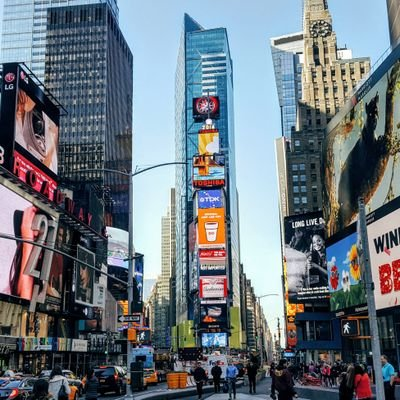
\includegraphics[width=0.45\textwidth]{tsq.jpg}
  \caption{Image to compress using k-means}
  \label{fig:times}
\end{figure}

\end{description}
\newpage
\textbf{Questions:}



\begin{problem}{15}\textbf{K-means:}
\begin{description}
\item[(5) a.] K-means is a simple unsupervised learning algorithm that splits the data into clusters. There are different ways to determine the ``optimal'' number of clusters; the elbow rule being a very simple one. Explain it in at most 4 sentences.
\item[(5) b.] The pairwise objective gives the total pairwise distance of points within each cluster.  Here is the pairwise loss with squared Euclidean distance and $K$ clusters $c_1,c_2...c_K$:

$$W(c_1,c_2,...c_K) = \sum_{k=1}^K \sum_{i:c_i = k} \sum_{j:c_j = k} ||x_i -x_j||^2$$

The centroid objective gives the total distance of points from the centroid of each cluster.  Here is the centroid loss with squared Euclidean distance and $K$ clusters $c_1,c_2...c_K$:

$$F(c_1,c_2,...c_K)=\sum_{k=1}^K \sum_{i:c_i = k} ||x_i - \bar{x}_k||^2$$
where 
$$\bar{x}_k = \frac{1}{N_k} \sum_{i:c_i = k} x_i$$

In lecture, Brendan claimed that the centroid loss is equivalent to the pairwise loss. Is this actually true?   In other words, does $W(c_1,c_2,..c_K) = F(c_1,c_2,..c_K)$ for any $K$ and any assignment of clusters? Prove your result.  

\item[(5) c.]Explain the relationship between pairwise loss and centroid loss.   Under what conditions you would expect them to give similar behavior?  Under what conditions would they give different behavior?
\end{description}
\end{problem}
\newpage
\begin{problem}{35}\textbf{K-means Image Compression:}
You are given an RGB image \textit{times\_square.jpg} as a $400 \times 400 \times 3$ matrix. Each pixel can be seen as a sample of dimension 3 (3 integers between 0 and 255, one for each component of RGB). For this question you will treat each pixel as a data sample. You are encouraged to use \textit{sklearn's} implementation of \textit{kmeans} for this question.

\begin{figure}[H]
  \centering
  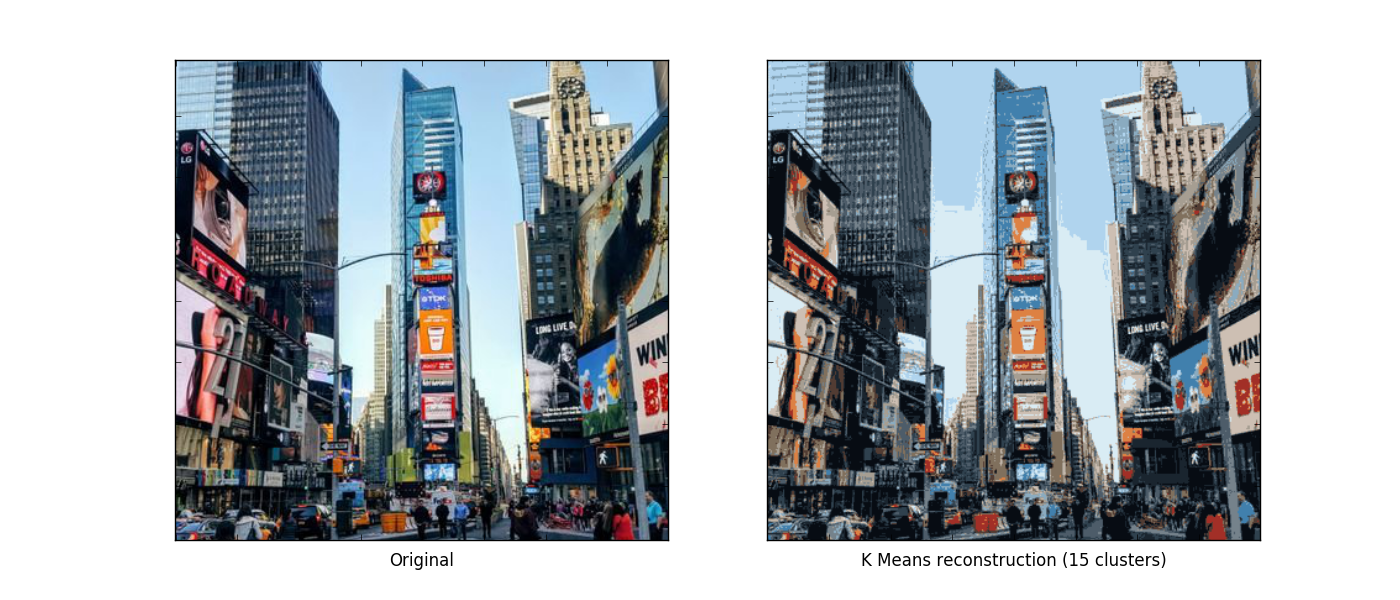
\includegraphics[width=6in]{kmeans_example15.png}
  \caption{Example of reconstructed image using 5 clusters}
  \label{fig:kmeans}
\end{figure}

\begin{description}
\item [(10) a.]Apply k-means using $k$ clusters in the range $\{2, 5, 10, 25, 50, 75, 100, 200\}$ (note that in this case each cluster will represent an RGB color triplet). Replace each pixel in the original image with the centroid of the cluster assigned to that pixel. In your report, make a $3 \times 3$ grid plot of the original times square image along with eight reconstructed images corresponding to eight different values of $k$. Make sure to label the images. An example of the original image and reconstructed image is shown in Figure \ref{fig:kmeans}. Helper code is given in `run\_me.py' file to convert the $400 \times 400 \times 3$ matrix to $160,000 \times 3$ matrix and vice versa.

\item [(10) b.]Make a plot of the sum of squared errors of each pixel to its respective cluster centroids for different values of $k$ (elbow plot). If the range is too big then make the plot in $\log$ space, but make sure to indicate that in your report.

\item[(2.5) c.]In at most three sentences, discuss and comment on your results from (a) and (b).  How does $k$ affect the quality of the reconstructed images?  How does SSE change with $k$?

\item [(10) d.]


 Another way to assess image compression is to look at the compression rate. The compression rate is the memory required to store the compressed image divided by the memory required to store the original image. Note that in this case each pixel of the original image uses 24 bits, each centroid is represented by 3 \textit{floats} (each one uses 32 bits), and an integer from 1 to $k$ needs $ceiling(\log_2k)$ bits (for each pixel in the image you store the index of the centroid assigned). For each value of $k$ report the compression rate using the table below. In python, you can use numpy's nbytes to get the number of bytes consumed by an array, vector, etc.


For each value of $k$, report the compression rate in a format like the table below.  


\begin{table}[H]
	\centering
	\begin{tabular}{|l|c|c|c|}
		\hline
		 & Compression Rate \\\hline
		$k = 2$		&            \\\hline
		$k = 5$     &            \\\hline
		$k = 10$		&            \\\hline
		$k = 25$    &            \\\hline
		$k = 50$    &            \\\hline
		$k = 75$    &            \\\hline
		$k = 100$  	&            \\\hline
		$k = 200$  	&            \\\hline
	\end{tabular}
\end{table} 
\item [(2.5) e.]In at most two sentences, describe and comment on your reported compression rates.  How does $k$ affect the compression rate?

\end{description}
\end{problem}

\showpoints
\end{document}

